\subsection{AES encryption round}

AES Encryption rounds consist of four transformations explained in previous sections. A circuit that can be used to implement a round is presented in figure \ref{fig:aes-round}.

\begin{figure}[!h]
\centering
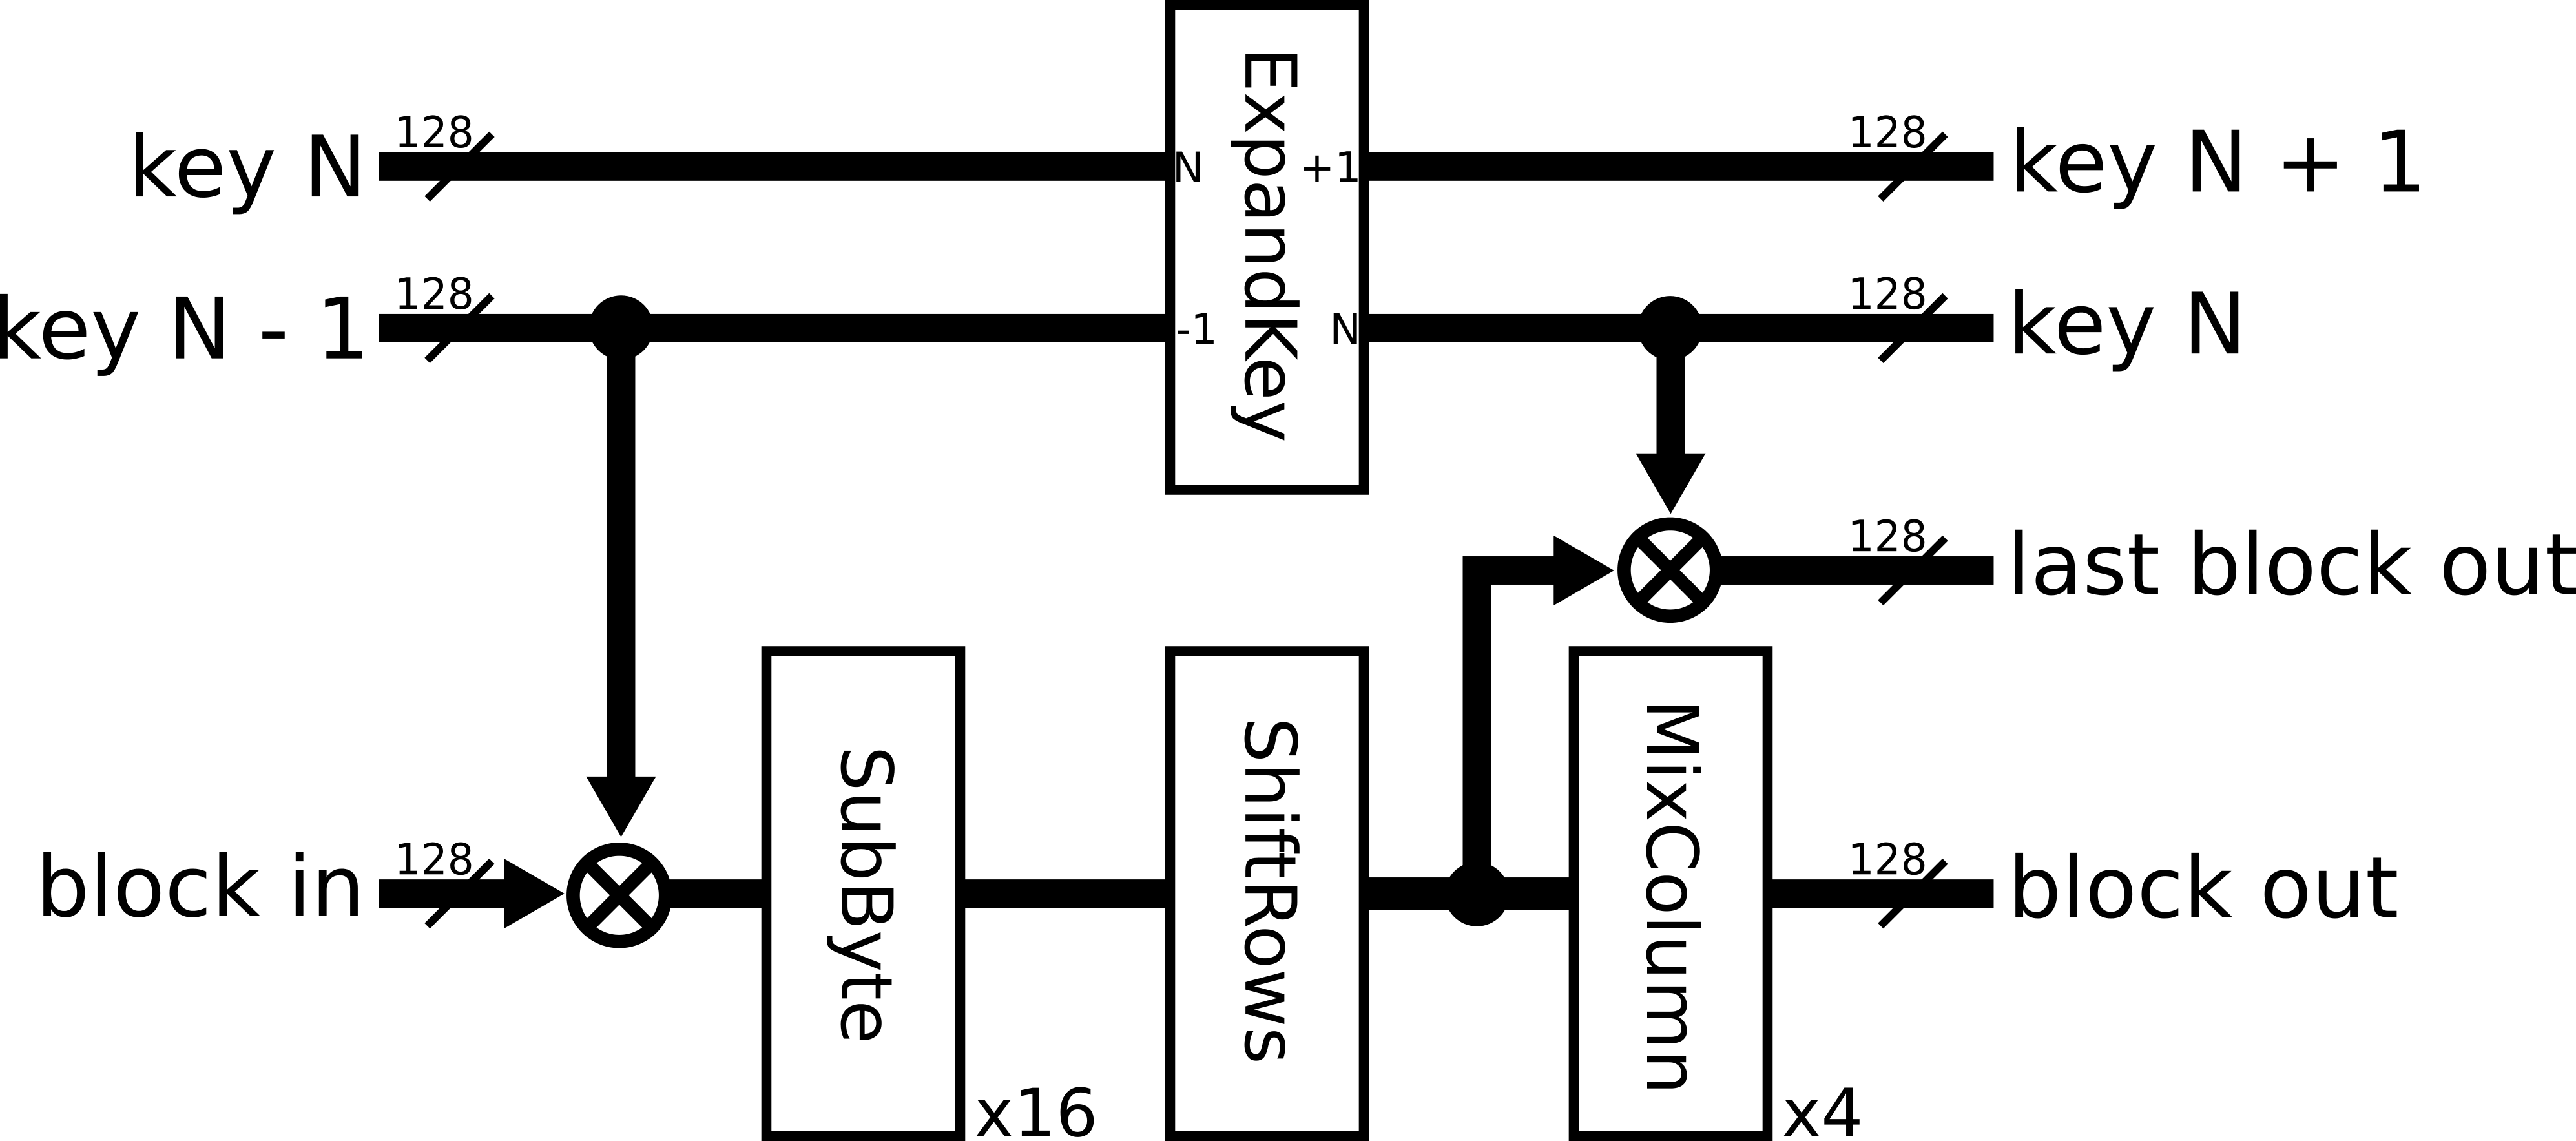
\includegraphics[scale=4]{aes-round}
\caption{AES round circuit}
\label{fig:aes-round}
\end{figure}

256-bit version of AES encryption algorithm, which is analysed here, has 15 rounds. Rounds 2 to 14 are the same and use all four transformations (fig. \ref{fig:aes-round}). First round only applies AddRoundKey transformation to the state. Last round is similar to rounds 2 to 14, but it does not apply MixColumns transformation.

